\documentclass{article}
\usepackage{amsmath}
\usepackage{bm}
\usepackage{graphicx}
\usepackage{float}

\begin{document}

\title{Intermediate Report}

\author{Nicolas Bougie, Nawel Medjkoune, Stephen Batifol,\\ Abdelhadi Temmar, and Abdoun Sihem}
\maketitle



\section{Introduction}

\subsection{Project Context}


For this project, we had to work on evolution algorithms that are commonly applied to black-box optimization problems. From the algorithm pointview, evolution strategies are optimization methods that sample new candidates solutions stochastically.
One had to implement a chosen algorithm described in \cite{DBLP:reference/sp/HansenAA15}, we chose to implement the given algorithm with Python. The algorithm had his parameter control via self-adaptation. One had then to run a suite of test functions in order to benchmark the performance of the implemented algorithm.  As central performance measure of algorithms COCO compute the "runtime" measured by the number of evaluations performed on the problem. In other words "runtime" is defined by the number of calls to the objective function until a target value is hit. This performance measure is independent from the used programming language and the material running the algorithm.



\subsection{Project Goals}
In order to know which algorithm to use for a particular numerical black-box optimization problem, we have to benchmark multiple algorithms. For this particular project, we have implemented   $(\mu / \mu \overset{+}{,} \lambda)-ES$ \cite{DBLP:reference/sp/HansenAA15}, a non-benchmarked algorithm and benchmarked it with COCO \cite{DBLP:journals/corr/HansenAMTB16}. We can then compare our implementation of this algorithm with another group that implemented the same algorithm but with another programming language. Finally, we compare this algorithm with two  baseline algorithms, BIPOP-CMA-ES \cite{hansen2009benchmarking} and BFGS \cite{ros2009benchmarking}.

In this intermediate report, we state our progress during the first part of the project. In section 2.1, we explain the algorithm implemented and give the pseudo-code. In section 2.2, details about implementation are explained. In section 2.3, the algorithm integration in COCO is detailed. In section 2.4, we sum up the preliminary experiments configuration. Results are shown and discussed in section 2.5 and suggestion about further investigation are given. We state some of the encountered difficulties during implementation in the next section. Finally, in section 3, we sum up what remains to be done in the project.


\section{Progress state}

\subsection{Understanding the algorithm}
The algorithm studied in this project is $(\mu / \mu \overset{+}{,} \lambda)-ES$ \cite{DBLP:reference/sp/HansenAA15}. Prior to implement the algorithm, we first had to understand it. We proceeded by understanding what an evolutionary algorithm consist of and the mechanism behind the template 2 of the paper which corresponds to the pseudocode of the evolution strategy that is used in the article.

First of all, evolutionary algorithms are a set of algorithms inspired from the theory of biological evolution frequently used to solve optimizations problems. These algorithms are most commonly population-based where each individual of the population is considered as a candidate solution to the problem and its quality is measured by a loss function (objective function). 
The concept of the algorithm is close to biological evolution and Darwin’s theory. The initial population is randomly generated (origin of life). This population has a very low evaluation score and is weak (relative to survival). The offsprings (second generation) are generated from one or several parents. These descendants inherit genes from their parents and then mutate their genes . Only the strongest individuals survive (the ones with the best evaluation score). This leads to a stronger and stronger population, in other words : get closer to the optimal solution.
The purpose is then to improve the solutions iteratively by generating new solutions through stochastic mechanisms such as: selection, recombination or mutation.  

\begin{figure}[H]
\begin{center} 
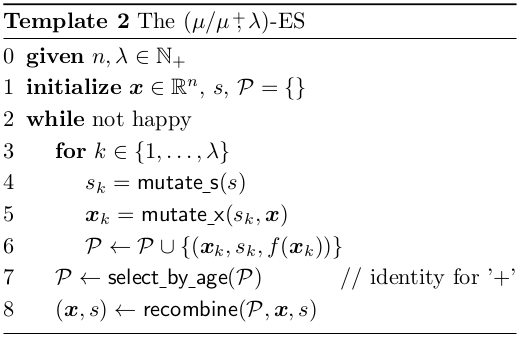
\includegraphics[scale=0.5]{figures/temp2.png}
\caption{Template 2}
\label{template2}
\end{center}
\end{figure}


Figure \ref{template2} shows the template 2 exposed in the paper. The particularity of this template is the use of a single parental centroid $(x, s)$, which simplify the algorithm. We shall use this single parental centroid to create a new generation of offspring. $S_{k}$, more commonly called "standard deviation",  is used to generate a new offspring $X_{k}$. Intuitively, The bigger $S_{k}$ is, the bigger the distance between $X$ and $X_{k}$ is. This is why $\sigma$ and $\sigma_k$ change through iteration, we want this parameter to adapt over time, this process is called Self Adaptation.
We use $X$ and $S$ to generate the set $(x_{k}, s_{k}, f(x_{k}))$ for $k = [0, \lambda]$. At line 6 and 7, the population is updated using the new samples. At line 8, $X$ and $S$, the parental centroid, is updated.


\begin{figure}[H]
\begin{center} 
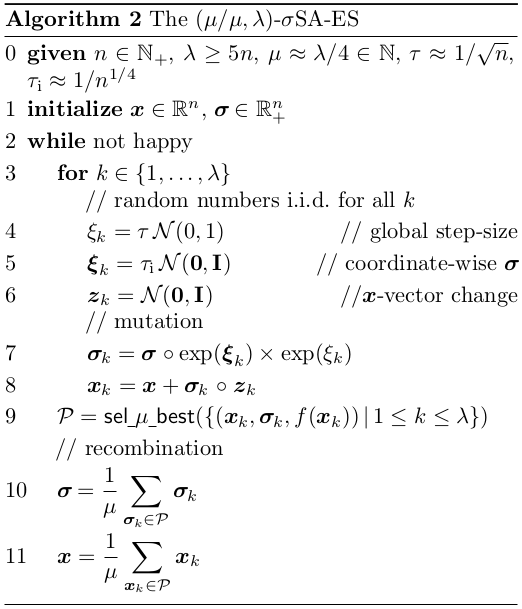
\includegraphics[scale=0.5]{figures/algo2.png}
\caption{Algorithm 2}
\label{algorithm2}
\end{center}
\end{figure}


Figure \ref{algorithm2} shows the pseudocode of the $(\mu / \mu \overset{+}{,} \lambda)-ES$ algorithm. The goal of the algorithm is to minimize a black box function. More precisely, the algorithm tries to find a $X$ (entry of $f$) which will minimize $f(X)$. For this reason, we first have to initialise randomly $X$ and try to find near this parental centroid a better solution.
To understand this algorithm, we need to understand how the mutation, selection and recombination are made.
First of all, the mutation. During this step, we create a new generation ($\lambda$ childs) by applying random changes following a normal distribution. We can see at line 7, that we apply 2 to \bm{$\sigma$}. One mutation who is common to all components of the vector (the scalar computed at line 4), and one who is different for each component of \bm{$\sigma$} (the vector computed at line 6). For $x$, we apply a different mutation for each component (line 8). The sign of $\sigma_{k} \circ z_{k}$ will indicate for each component of $X$ which direction to follow. 


Once the mutation is done, we shall do the selection. Individual’s selection is done by taking the µ best individuals among the lambda individuals of the new generation. In this algorithm we let individuals die after one iteration. 

The recombination is simple. We compute the average of the new population to update the parental centroid (line 10, 11). 
However, the application of mutation and recombination introduces a moderate bias such that $\sigma$ tends to increase.

In order to achieve stable behavior of $\sigma$, the number of parents $\mu$ must be large enough, which is reflected in the setting of $\lambda$.


\subsection{Algorithm Implementation and General Code Structure}

Prior to implementing the algorithm, several questions were raised:
\begin{enumerate}
\item How do we initialize $X$ and $\sigma$?
\item When do we stop the algorithm?
\item How do we choose the value of $\lambda$?
\item What budget do we choose?
\end{enumerate}

These are not trivial choices that can be decided with theory only. Experiments need to be done in order to make the best decisions. 


For now, we decided to initialize $X$ between $-5$ and $5$ because according to the bbob dataset documentation,the optimum is always between $-5$ and $5$. $\sigma$ is initialized between $0$ and $0.01$ to start with a small value. This choice was made because we know that the optimum is between $-5$ and $5$. Therefore, we do not need a big standard deviation. 

The current implementation of the algorithm stops only when no budget is left, to see where the algorithm can go. In the future, the algorithm will stop itself when it finds a solution equals or smaller than the target objective.

Lambda is currently set to $5*n$, where $n$ is the size of the vector $X$. It is the minimum value advised by the authors of the paper. In the future, we will try to change that value, to see if it affects the results.

We try to test our algorithm with multiple budgets to see for which values the algorithm converges.


\subsection{Algorithm integration in Coco}

Coco is a platform for comparing continuous optimizers in a black-box setting. 
Coco provides an interface to run our own optimizer. We first changed the search space also called "dim" . We chose different dimensions to see if the algorithm could efficiently find a "good" solution in a higher dimension. We benchmarked our implementation of the algorithm on  the BBOB suite, which  contains mono objective and noiseless functions [REF].

The optimizer is called from the run$\_$optimizer function. This function takes as parameters the evaluation function, the dimension of the search space, the maximum number of evaluations and the optimal solution. These values are provided by COCO. Inside this function, the parameters specific to our algorithm are generated. Then, we call our optimizer with all the previous parameters.

We also set the budget (maximum number of evaluations), we chose a small value to accelerate the computations.
Our function does not need to be modified. It just returns the best solution and check that the number of evaluation is not exceeded. 
Coco automatically measures the performances for each problem and generate a folder containing the output.  

Coco also provides a LateX template to display a summary for the single-objective BBOB suite and algorithm performances.


\subsection{Experiments configuration}
To sum up what has been said before, we present the overall configuration for the preliminary experiments. We ran the algorithm $(\mu / \mu \overset{+}{,} \lambda)-ES$  on the BBOB noiseless functions test suite over different configuration settings: first of all, for the purpose of debugging and understanding the algorithm behaviour, we experimented relatively small values of budget and dimension. We tested three different budgets (500, 1000, 5000) with three different dimensions (2,3,5). The algorithm  $(\mu / \mu \overset{+}{,} \lambda)-ES$ was implemented in Python. The initial solution is generated randomly in $[-5,5]$ Dim  and a very small value for sigma is generated randomly as well. The parameter $\lambda$ is initially set to $5*dim$ and $\mu$ is one fourth of $\lambda$ according to the paper. Finally, the maximum number of runs (restarts) in set to its default value: $1e9$.


\subsection{Results and comments}
Results from our preliminary experiments are shown in the next figures. Figure \ref{fig1} represents runtime distribution (ECDFs) over all functions, targets and instances.

\begin{figure}[H]
\begin{center} 
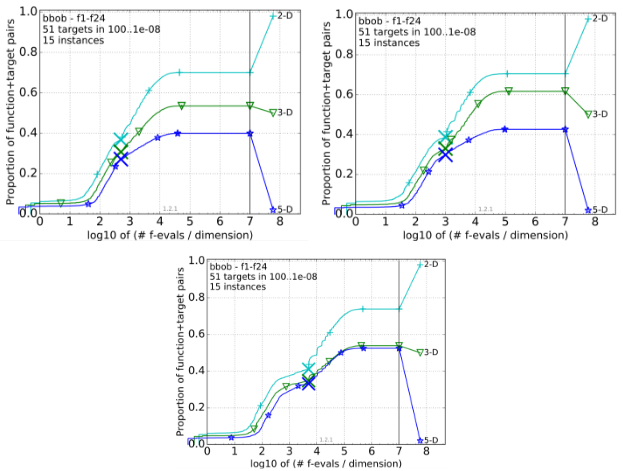
\includegraphics[scale=0.5]{figures/graphs1.png}
\caption{Runtime distributions (ECDFs) over all targets with budget=500, 1000, 5000 from left to right.}
\label{fig1}
\end{center}
\end{figure}

We observe that the algorithm with this configuration barely reaches 40\% of success over all the problems. However, we notice that the proportion of the problems solved increases slightly when the budget is increased. This observation is a motivation to go deeper in the experiments and test even bigger budgets. 
For the remaining discussion, we consider the results from the last run (i.e. with the budget of 5000 and dimension of 5).



\begin{figure}[H]
\begin{center} 
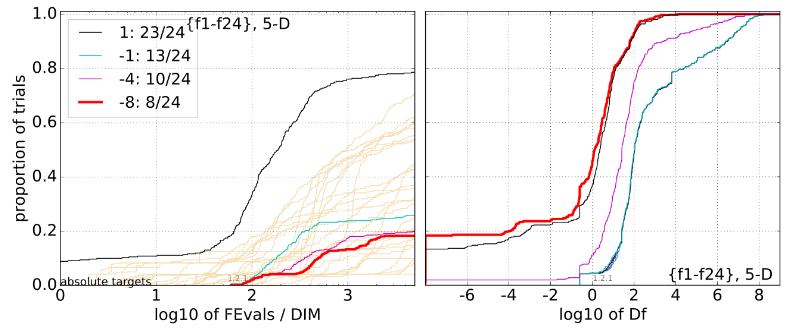
\includegraphics[scale=0.4]{figures/graphs2.png}
\caption{left: runtime distributions (ECDFs) for selected targets (precision), right: Legends indicate for each target the number of functions that were solved in at least one trial within the displayed budget.}
\label{fig2}
\end{center}
\end{figure}


In figure \ref{fig2}, we can observe the overall performance of the algorithm on all the functions depending on the target precision. For large precisions (i.e. $\Delta f = 101$), most of the problems are solved. The less the precision is, the worst the algorithm performance is. This problem needs to be investigated in the second half of the project. First suggestion is to allocated bigger values for the budget. Another suggestion is to vary the values of multiple input parameters of the algorithm and try other initialisation types. 
However, the algorithm performance over difficult precisions is still good when compared to the BBOB 2009 benchmarking results (light brown lines)

\begin{figure}[H]
	\begin{center} 
		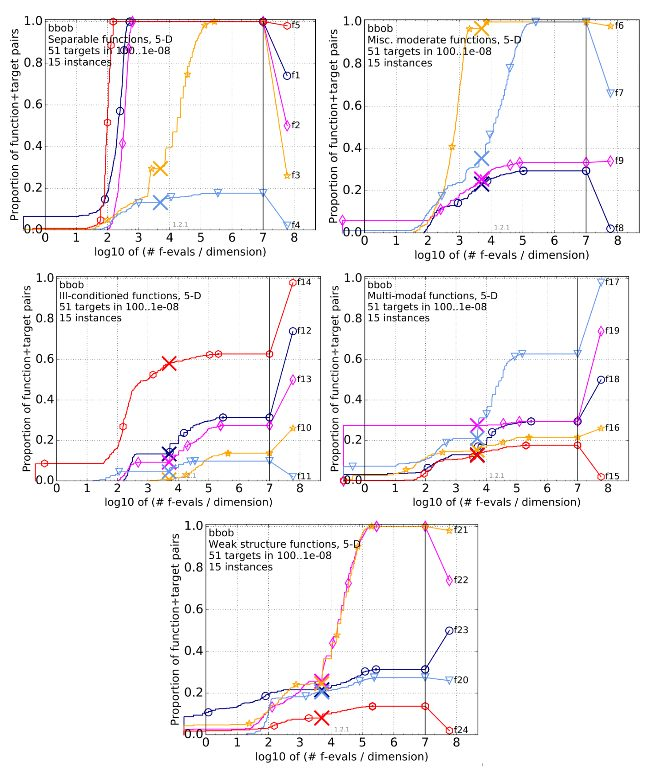
\includegraphics[scale=0.5]{figures/graphs3.png}
		\caption{Runtime distributions (ECDFs) per group and per function over all targets (dimension=5)}
		\label{fig3}
	\end{center}
\end{figure}


Figure \ref{fig3} shows ECDFs per groups for dimension 5. For the first group, 3 functions out of 5, as well as one function in the second group, are 100\% solved in the allowed budget. That said, most of the remaining problems, especially for the multi-modal and weak structure functions, do not exceed the 30\% threshold. Undoubtedly, problems with small precision are the ones that are solved unsuccessfully. 



Our main point of investigation for the future is, as said earlier, trying to increase maximum budget allowed and observe the results. Bigger dimensions have to be investigated as well.


\subsection{Encountered difficulties}
When we implemented the first version of   $(\mu / \mu \overset{+}{,} \lambda)-ES$ , we made some experiments with small values for the budget and dimensions, in the purpose of debugging our code. This method proved to be useful since we noticed very poor proportion of solved problems (which was strange for the separable functions) and some inconsistencies on the plots. Despite the few coding errors we patched, another modification was to change the initialisation pattern of solutions from completely random to a uniform distribution in $[-5,5]^{Dim}$ as suggested in the COCO documentation. This modification improved significantly the results.



\section{Remaining work}
In order to complete this project, we shall carry more experiments with more iterations. Because we only tested if our algorithm was correct and our understanding of COCO, we only allocated a maximum budget of 5,000. Our objective is to test our algorithm on a budget as high as 50,000. With this budget, we could compare our results with the ones produced previously on the BBOB serie. 
Another task would be to compare our implementation with the implementation of an other group. We could also vary the offspring population size to assess the impact of this variable on the results


\subsection{Go deeper in the experiments}
As suggested in the article, the change of the population size parameters $\mu$ and $\lambda$ has a significant impact on the search characteristics of an evolution strategy. We will carry multiple experiments in order to investigate the impact that these parameters will have on the algorithm performance.



\subsection{Comparing results with other algorithms}
As mentioned above, we chose the Python programming language to implement the chosen algorithm. Since there is another group working on the same algorithm but in C/C++, it would be interesting to compare our respective algorithms on the basis of their performance. Two baseline algorithms, namely BIPOP-CMA-ES \cite{hansen2009benchmarking} and BFGS \cite{ros2009benchmarking}, are also used for the comparison. 



\section{Conclusion}
As a conclusion for the first part of this project, we can say that we understood how COCO works and how it benchmarks algorithms. With the work done so far, we also understood what an evolutionary algorithm is and how it works and how to deal with numerical black-box optimization problems. 
As previously stated, for the remaining part of this project, we want to run our algorithm with a higher budget, we also want to change the population size parameters to investigate the impact that they will have on the algorithm performance.


As mentioned before, compare our algorithm with other evolutionary algorithms is crucial. We could compare it with different optimisation techniques such as particle-swarm, differential evolutions or variable-neighborhood search.






\bibliographystyle{apalike}
\bibliography{biblio-bibtex}

\end{document}